\documentclass[compress]{beamer}
\usepackage{ifthen,verbatim}

\newcommand{\isnote}{}
\xdefinecolor{lightyellow}{rgb}{1.,1.,0.75}
\xdefinecolor{lightgrey}{rgb}{0.9,0.9,0.9}
\xdefinecolor{darkblue}{rgb}{0.1,0.1,0.7}

\setbeamertemplate{navigation symbols}{}
\setbeamertemplate{headline}{\mbox{ } \hfill
\begin{minipage}{5.5 cm}
\vspace{-0.75 cm} \small
\end{minipage} \hfill
\begin{minipage}{4.5 cm}
\vspace{-0.75 cm} \small
\begin{flushright}
\ifthenelse{\equal{\insertpagenumber}{1}}{}{\insertpagenumber\isnote/\pageref{numpages}}
\end{flushright}
\end{minipage}\mbox{\hspace{0.2 cm}} \hspace{0.01 cm} \vspace{-1.05 cm}}

\begin{document}
\begin{frame}
\vfill
\begin{center}
\textcolor{darkblue}{\Large The Role of the Large Hadron Collider (LHC) \\ \vspace{0.2 cm} in the Quest to Understand Matter}

\vfill
\begin{center}
\large
\textcolor{darkblue}{Jim Pivarski}
\end{center}

\begin{columns}
\column{0.225\linewidth}
\mbox{ }

\column{0.125\linewidth}
\includegraphics[width=\linewidth]{../tamulogo}

\column{0.4\linewidth}
\begin{center}
\begin{minipage}{0.75\linewidth}
\begin{center}
\scriptsize {\it Texas A\&M University}

\vspace{0.2 cm}
{\it and a member of the CMS Collaboration (experiment at the LHC)}

\mbox{ }
\end{center}
\end{minipage}
\end{center}

\column{0.125\linewidth}
\includegraphics[width=\linewidth]{../cmslogo}

\column{0.225\linewidth}
\mbox{ }
\end{columns}

\vfill
25 February, 2009

\end{center}
\end{frame}

\small

\begin{frame}

\only<2>{\vspace{-0.7 cm}}
\begin{center}
\includegraphics[width=0.9\linewidth]{cernpanorama.jpg}
\end{center}

\only<2>{\vspace{-4.3 cm}
\hfill \mbox{ } \includegraphics[width=0.5\linewidth]{news1.png}}
\end{frame}

\begin{frame}
\frametitle{What's the big deal?}

\begin{itemize}\setlength{\itemsep}{0.3 cm}
\item Highest-energy collisions ever made by humans in a laboratory
\begin{itemize}\setlength{\itemsep}{0.1 cm}
\item on December 18, 2009: 2.36~TeV
\item previous record: 1.96~TeV (Fermilab Tevatron, 1987--now)
\item sometime next month: 7~TeV
\item after 2011 upgrade: 14~TeV
\end{itemize}

\item World's largest scientific experiment (not counting moon landing)
\begin{itemize}\setlength{\itemsep}{0.1 cm}
\item accelerators became too large for a single college campus in the mid-20$^{\scriptsize th}$ century
\item this is the first that is too large for a single nation: the first ``world's accelerator''
\end{itemize}

\item Long-anticipated: plans began in the mid-1970's

\item Why do we need such high-energy collisions?  \\ What can we learn from them?
\end{itemize}
\end{frame}

\begin{frame}
\frametitle{The LHC in context}
\only<1>{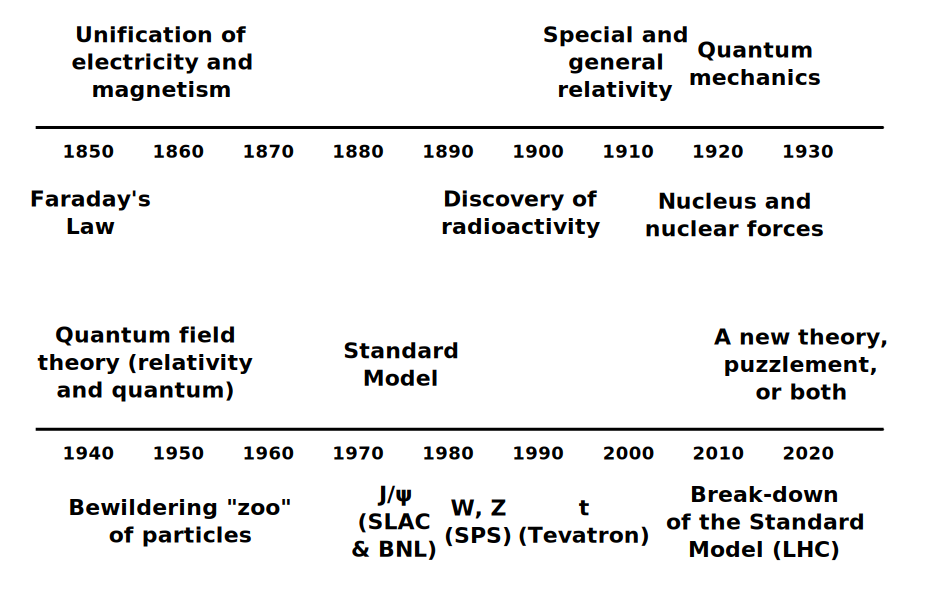
\includegraphics[width=\linewidth]{timeline.png}}
\only<2>{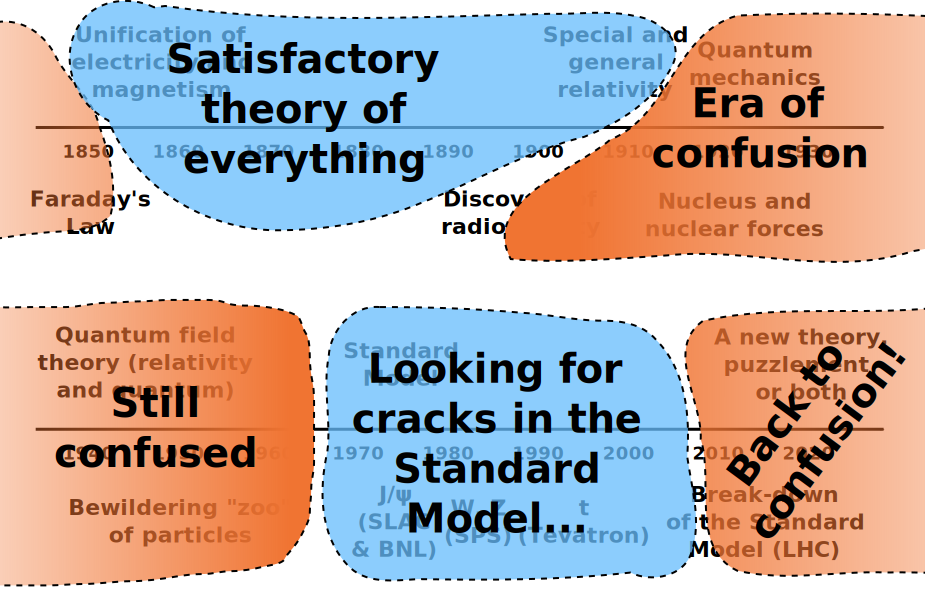
\includegraphics[width=\linewidth]{timeline_withblobs.png}}
\only<3>{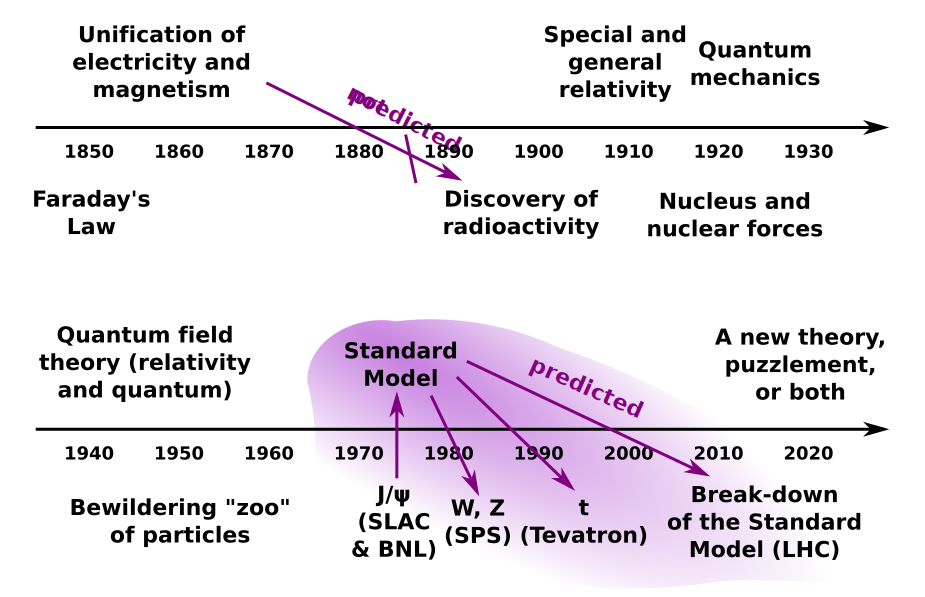
\includegraphics[width=\linewidth]{timeline3.png}}
\end{frame}

\begin{frame}
\frametitle{Color scheme for this talk}
\includegraphics[width=\linewidth]{timeline4.png}
\end{frame}

\beamertemplateshadingbackground{lightyellow}{lightyellow}
\begin{frame}
\frametitle{Electricity and magnetism}

\begin{itemize}
\item Field concept: every point in space (and time) has associated
  with it an electric field $\vec{E}$ (a vector; three numbers) and
  magnetic field $\vec{B}$

\item These numbers describe the local conditions at that position in
  terms of the force felt by a bit of matter with charge $q$, velocity $v$

\[ \vec{F} = q \left(\vec{E} + \vec{v} \times \vec{B} \right) \]

\item The field obeys certain transformation rules when changing
  coordinate systems and is the solution to a set of equations

\end{itemize}

\includegraphics[height=3.4 cm]{electric_field_lines.jpg} \hfill
\includegraphics[height=3.4 cm]{magnetic_lines_2010.png}
\end{frame}

\beamertemplateshadingbackground{lightgrey}{lightgrey}
\begin{frame}
\frametitle{How the LHC accelerates protons}

\begin{itemize}
\item A postively-charged proton feels a force $\vec{F} = q\vec{E}$ in
  a strong electric field $\vec{E}$ and undergoes acceleration
  $\vec{a} = \vec{F}/m$ ($m = \mbox{proton mass}$)

\item Technical challenge: creating strong fields $\vec{E}$

\item Solution: strong {\it oscillating} fields can be produced with
  radar towers and piped into resonating cavities.  A pulsed beam is timed to
  enter each cavity exactly when the field is pointing in the right
  direction to accelerate it, rather than decelerate it.
\end{itemize}

\includegraphics[height=4 cm]{lhc_rf_cavity.jpg} \hfill
\includegraphics[height=4 cm]{rf_cavity.jpg}
\end{frame}

\begin{frame}
\frametitle{How the LHC contains proton beams}

\begin{itemize}
\item Constant magnetic field $\vec{B}$ yields $\vec{F} = q\vec{v} \times \vec{B}$ (``right-hand rule'')

\item Challenge: strong $\vec{B}$.  Solution: ultra-high current
  electromagnets made from superconducting wires (no losses due to
  resistance)
\end{itemize}

\includegraphics[height=6 cm]{lhc_dipole.jpg} \hfill
\includegraphics[height=6 cm]{cernpanorama_bfield.jpg}
\end{frame}

\beamertemplateshadingbackground{lightyellow}{lightyellow}
\begin{frame}
\frametitle{Quantum field theory}
\begin{center}
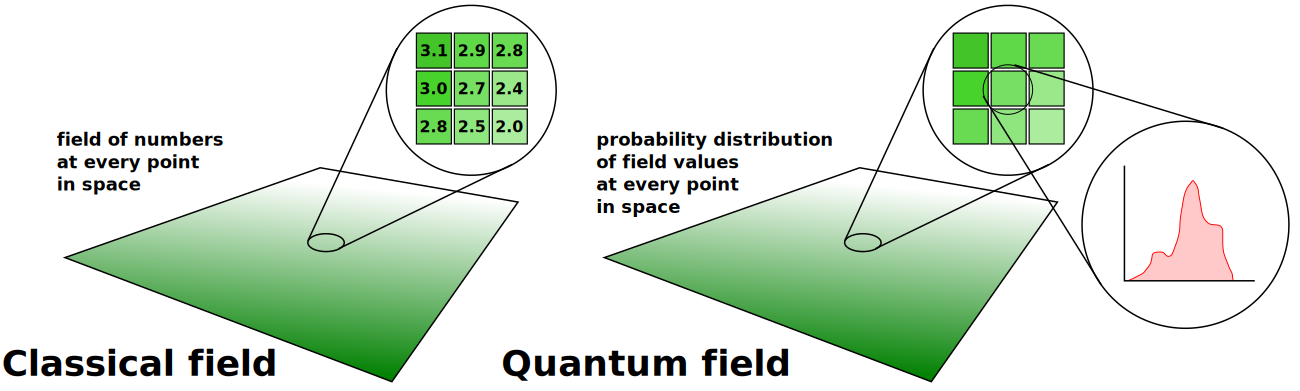
\includegraphics[width=0.9\linewidth]{classical_quantum_fields.png}
\end{center}

\begin{itemize}
\item No distinction between fields and matter: everything's a field

\item Quantum field: {\it probability distribution} of values at each
  point in space-time, with correlations between neighboring points

\item Consequence: energy of field configuration is {\it quantized} into
  integers--- zero particles, one particle, two particles\ldots
\end{itemize}

\includegraphics[width=\linewidth]{fieldvalues.png}
\end{frame}

\begin{frame}
\frametitle{Quantum field theory}

\begin{itemize}
\item \bf Consequence: energy of field configuration is quantized into
  integers--- zero particles, one particle, two particles\ldots
\end{itemize}

\includegraphics[width=\linewidth]{fieldvalues.png}

\begin{itemize}
\item What we call ``empty space'' is the minimum-energy fluctuation of
  the field; what we call ``a particle'' is the first excitation

\item For each fundamental type of particle, there is a distinct
  field; \\ what we call a photon is a single excitation of the photon
  field, \\ an electron is an excitation of the electron field, etc.

\item<2> Why quantized?  $\displaystyle i \sqrt{-\left(\frac{\partial \Psi}{\partial x}\right)^2 + \left(\frac{\partial \Psi}{\partial t}\right)^2}
= \left( -\frac{1}{2}\frac{\partial^2}{\partial \phi^2} + m^2 \phi^2 \right) \Psi$

is a seperable equation where $\left|\Psi(\phi; x, t)\right|^2$
is the probability density of field values $\phi$ at space-time
points $x$, $t$
\end{itemize}
\end{frame}

\beamertemplateshadingbackground{lightgrey}{lightgrey}
\begin{frame}
\frametitle{Detecting individual particles at the LHC}

\begin{itemize}
\item A single high-energy charged particle pulls the electrons off of
  neutral atoms as it passes by; this released charge is collected
  onto wires and read into a computer

\item Pattern of observed hits line up as a track, indicating
  the trajectory of the original high-energy particle

\item Below: a muon from space passing through the CMS silicon
  tracker, with a strong magnetic field in the $\hat{z}$ direction (see the curvature?)
\end{itemize}

\vfill
\includegraphics[height=3.7 cm]{cosmic_event.png} \hfill
\includegraphics[height=3.7 cm]{tracker.jpg}
\end{frame}

\beamertemplateshadingbackground{lightyellow}{lightyellow}
\begin{frame}
\frametitle{Creating and destroying particles}

\begin{itemize}
\item Fields are {\it coupled} to each other, allowing energy to flow
  from one field into another
\item Massive particles can decay into lighter particles, converting
  the leftover mass into kinetic energy of the decay products
\item The probability of decay depends on the strength of the coupling
\end{itemize}

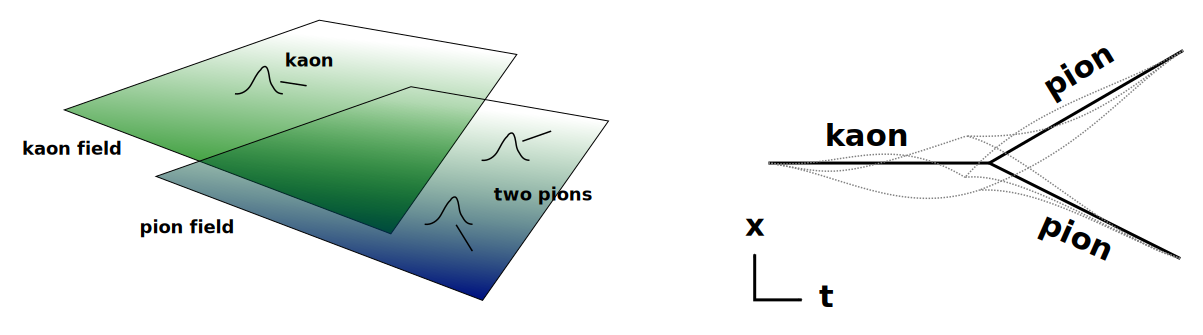
\includegraphics[width=\linewidth]{ktopipi_fields.png}

\begin{itemize}
\item It also works in reverse: colliding two protons at 14~TeV allows
  anything to be created that satisfies all conservation rules--- any
  new particle with mass at most 14~TeV/$c^2$, or several particles
\end{itemize}
\end{frame}

\beamertemplateshadingbackground{lightgrey}{lightgrey}
\begin{frame}
\frametitle{Creating particles in proton collisions}

Photo from an old \hfill Reconstructed LHC event, \\
bubble chamber, \hfill December 18, 2009 \\
identified by hand

\vspace{0.2 cm}
\includegraphics[height=4.5 cm]{k0-to-pipi_bubblechamber.png} \hfill
\includegraphics[height=4.5 cm]{cms_kshort.png}

\vspace{0.2 cm}

Proton beam (upward) \hfill Proton beams are perpendicular to this \\
on liquid containing \hfill projection before collision; newly-created \\
protons (stationary) \hfill particles go everywhere
\end{frame}

\begin{frame}
\frametitle{Identifying particles by their decays}

\begin{columns}
\column{0.5\linewidth}
\includegraphics[width=\linewidth]{cms_kshort.png}

\begin{itemize}
\item Neutral kaon leaves no track
\item Energy $E$ and momentum $\vec{p}$ are conserved in the decay
\end{itemize}

\column{0.5\linewidth}
\includegraphics[width=\linewidth]{kshort-distribution.png}
\end{columns}

\vspace{0.3 cm}
\hspace{1 cm} $(E)^2 = (mc^2)^2 + |\vec{p}|^2c^2$

\vspace{0.2 cm}
\mbox{\hspace{-0.45 cm}
\begin{minipage}{1.05\linewidth}
\begin{itemize}
\item Add up the energies and momenta of the pion pairs and solve for $m$, \\ for all pairs of observed tracks
\begin{itemize}
\item in the statistical distribution, true kaons peak at $m$, the kaon mass
\item false combinations, {\it or background,} are more uniformly distributed
\end{itemize}
\end{itemize}
\end{minipage}}
\end{frame}

\beamertemplateshadingbackground{lightyellow}{lightyellow}
\begin{frame}
\frametitle{Forces in quantum field theory}
\begin{itemize}
\item Quantum field theory explains how particles are created from
  kinetic energy and how they can decay into other types of particles

\vspace{0.25 cm}
\item Also describes forces, e.g.\ repulsion of two electrons:

\vspace{0.5 cm}
\begin{columns}
\column{0.5\linewidth}
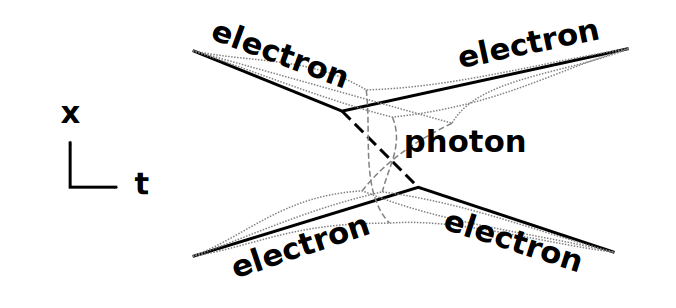
\includegraphics[width=\linewidth]{forces.png}
\column{0.5\linewidth}
\scriptsize
Two electrons are initially approaching each other, one of them
creates a photon and recoils because of the momentum it gave to the
photon, then the photon is absorbed by the other electron, which
recoils when it accepts that momentum.
\end{columns}

\vspace{0.5 cm}
\item Goal of particle physics: to discover and understand all of the
  matter fields (like electrons) and all of the force fields (like
  photons) in a unified framework

\item How many forces are there, anyway?
\end{itemize}
\end{frame}

\beamertemplateshadingbackground{lightgrey}{lightgrey}
\begin{frame}
\frametitle{The fundamental forces}
\begin{itemize}\setlength{\itemsep}{0.2 cm}
\item<1-> \textcolor{darkblue}{Electromagnetism:} fundamental cause of all
  attributes of matter known before 1896 (stickiness, repulsion,
  sparks, chemical properties, light, color, etc.), other than
  gravity

\item<2-> \textcolor{darkblue}{Strong nuclear force:} holds protons and
  neutrons together in atomic nuclei, usually.  When it fails to hold
  or is deliberately broken, it releases vast amounts of nuclear
  energy.  But it's also complicated, producing hundreds of distinct
  particles (today known to be groups of strongly bound quarks).

\item<3-> \textcolor{darkblue}{Weak force:} causes particles to decay with
  much lower probabilities than the strong force.  Standard Model
  unifies weak with electromagnetism (``electroweak'').

\item<4> \textcolor{darkblue}{Gravity:} has more to do with space-time
  itself than field values at space-time points.  Because the
  gravitational force between microscopic particles is so small, the
  quantum nature of gravity can't be experimentally studied in
  particle collisions.
\end{itemize}
\end{frame}

\beamertemplateshadingbackground{lightyellow}{lightyellow}
\begin{frame}
\frametitle{The Standard Model}

All known fields and their couplings:
\begin{center}
\includegraphics[width=0.6\linewidth]{standard_model.png}
\end{center}

\begin{itemize}
\item Electromagnetic is the photon part of the diagram
\item Electroweak is photon, W boson, and Z boson
\item Strong nuclear force is the quark/gluon part
\end{itemize}
\end{frame}

\begin{frame}
\frametitle{The Standard Model}

All known fields and their couplings:
\begin{center}
\includegraphics[width=0.6\linewidth]{standard_model.png}
\end{center}

\begin{itemize}
\item Electroweak couplings are approximately equal, but
  electromagnetic interactions are far more common in everyday life than weak ones.
\item Standard Model explanation: W and Z mass is a trillion times higher
  than room-temperature energy, and the probability to create an
  intermediate W/Z is correspondingly small
\end{itemize}
\end{frame}

\begin{frame}
\frametitle{The Standard Model}

All known fields and their couplings:
\begin{center}
\includegraphics[width=0.6\linewidth]{standard_model.png}
\end{center}

\begin{itemize}
\item Technical problem: in quantum field theory, mass of matter
  fields (boxes) can simply be part of the equations describing the
  fields

but force fields (ellipses), must have zero mass in the wave equation!

\item Solution: take a hint from the strong nuclear force\ldots
\end{itemize}
\end{frame}

\begin{frame}
\frametitle{Masses in the strong nuclear force}

\hfill \includegraphics[height=3 cm]{strong_force.png} \hspace{1 cm} \includegraphics[height=3 cm]{inside_proton.png}

\vspace{-3 cm}
\begin{itemize}
\item Nuclear force has \\
a large coupling \\
and a self-coupling

\item Intermediate \\
gluons spawn more \\
gluons and more \\
gluons\ldots

\item Mass of three quarks in a proton is about 1\% of the proton mass

\item 99\% of the mass of protons, neutrons--- and therefore us--- is the
  potential energy of the attraction of the quarks to each other
  through gluons and the attraction of gluons to gluons

\item We are made of potential energy!
\end{itemize}
\end{frame}

\begin{frame}
\frametitle{Using this trick}

\begin{center}
\only<1>{\includegraphics[width=0.6\linewidth]{standard_model_whiggs.png}}
\only<2>{\includegraphics[width=0.6\linewidth]{standard_model_whiggs_quarkmass.png}}
\end{center}

\begin{itemize}
\item<1-> Don't give W and Z masses by hand, but let them be dynamically
  generated by interactions

\item<1-> Need to introduce a new particle to do it, a
  Englert-Brout-Higgs- Guralnik-Hagen-Kibble boson (``Higgs'' for short)

\item<1-> Now it's consistent

\item<2> Variant: explain all quark and charged lepton masses
  the same way
\end{itemize}
\end{frame}

\begin{frame}
\frametitle{Standard Model: a falsifiable hypothesis}

\begin{center}
\includegraphics[width=0.6\linewidth]{standard_model_undiscovered.png}
\end{center}

\begin{itemize}
\item When the Standard Model was proposed, the $W$, $Z$, and Higgs
  had not been observed as particles

\item The model predicts their properties (e.g.\ production rate in
  proton collisions and what they decay into)

\item If they are not discovered by a collider/detector which is
  sensitive to them, the model is wrong.  If they are discovered with
  the right properties, that's great evidence for the model.
\end{itemize}
\end{frame}

\beamertemplateshadingbackground{lightgrey}{lightgrey}
\begin{frame}
\frametitle{Long-term dreams: ``tens of TeV'' collisions are ideal}

{\it Popular Mechanics,} April 1978: early plans for LHC

\vfill
\includegraphics[width=\linewidth]{popular_mechanics.png}
\end{frame}

\begin{frame}
\frametitle{1980's: Super Proton Synchrotron at CERN}

\begin{itemize}
\item Collided protons and anti-protons at 0.9~TeV
\item Discovered $W$ and $Z$ bosons in 1983!
\item Now used to pre-accelerate protons into the LHC
\end{itemize}

\begin{center}
\includegraphics[height=4 cm]{ua2.jpg} \hspace{1 cm}
\includegraphics[height=4 cm]{happy_about_z_discovery.jpg}
\end{center}
\end{frame}

\begin{frame}
\frametitle{1990's: Tevatron at Fermilab (near Chicago)}

\begin{itemize}
\item Colliding protons and anti-protons at 1.96~TeV
\item Discovered $t$ quark in 1995
\item Two detectors on the same beamline; provides independent
  cross-checks when only one accelerator of this scale can be
  constructed
\end{itemize}

\vfill
\includegraphics[height=4.5 cm]{d0.jpg} \hfill
\includegraphics[height=4.5 cm]{cdf.jpg}
\end{frame}

\begin{frame}
\frametitle{2010's: LHC at CERN}

\begin{itemize}
\item Four detectors along the beamline; two are general-purpose
\end{itemize}

\begin{center}
\includegraphics[width=0.9\linewidth]{sun_shines_in_the_detector.jpg}
\end{center}
\end{frame}

\begin{frame}
\frametitle{2010's: LHC at CERN}
\includegraphics[width=\linewidth]{atlas.jpg}
\end{frame}

\begin{frame}
\frametitle{Berlioz's {\it Les Troyens}}
\includegraphics[width=\linewidth]{berlioz_troyens.jpg}
\end{frame}

\begin{frame}
\frametitle{What the $Z$ boson looks like}

Statistical mass distributions of $Z \to e^+e^-$ (with backgrounds):

\begin{columns}
\column{0.34\linewidth}
\begin{center}
Discovery
\end{center}
\includegraphics[width=\linewidth]{z_discovery.png}

\column{0.26\linewidth}
\begin{center}
Today (Tevatron)
\end{center}
\includegraphics[width=\linewidth]{cdf_23_zee.png}

\column{0.37\linewidth}
\begin{center}
Future (few months LHC)
\end{center}
\includegraphics[width=\linewidth]{InvMasse10_CORINNE.png}
\end{columns}

\vfill
\begin{itemize}
\item Discovery of massive W and Z with the right properties confirmed
  the Standard Model

\item High-precision studies in the 1990's makes the Standard Model
  one of the most precisely tested theories in physics

\item But\ldots\ no Higgs\ldots

\end{itemize}
\end{frame}

\begin{frame}
\frametitle{Why Higgs searches are hard}

\hfill 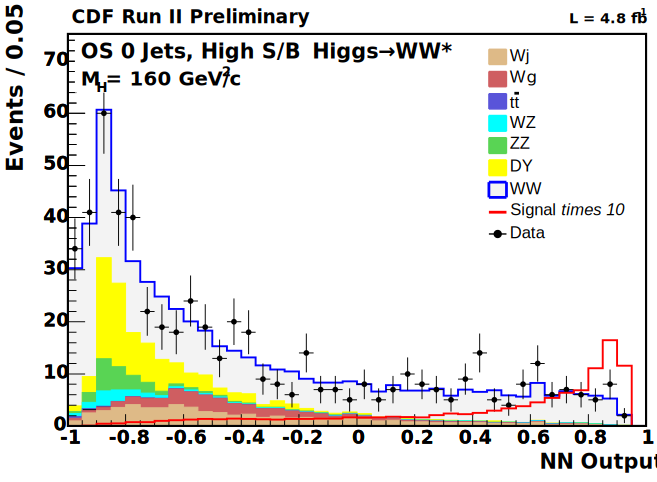
\includegraphics[width=0.5\linewidth]{tevatron_ww.png}

\vspace{-4 cm}
\begin{itemize}
\item A Higgs boson is probably \\
created once every few days \\
at the Tevatron, but it's \\
hidden under backgrounds

\item Many different types of \\
backgrounds

\item Applying artificial intelligence \\
algorithms (neural nets, etc.) \\
to distinguish signal from background using many variables
simultaneously, the way a human would

\item Example plot (one of the more promising modes):
  \textcolor{red}{signal} is multiplied by 10
\end{itemize}
\end{frame}

\begin{frame}
\frametitle{What can the Tevatron say about the Higgs?}

\begin{columns}
\column{0.55\linewidth}
\includegraphics[width=\linewidth]{fermilab_higgs_exclusion.png}

\vspace{0.2 cm}
\includegraphics[width=\linewidth]{probability_higgs_fermilab.png}

\column{0.45\linewidth}
\begin{itemize}
\item Top: which Higgs masses have been ruled out

\vspace{3 cm}
\item Bottom: probability of obtaining marginal evidence for a discovery, as a
  function of Higgs mass
\end{itemize}
\end{columns}
\end{frame}

\begin{frame}
\frametitle{LHC needed to definitively discover/rule out Higgs}

\begin{columns}
\column{0.6\linewidth}
Example signature only at LHC: Higgs \mbox{decaying into two photons\hspace{-5 cm}}

\begin{itemize}
\item Higgs does not couple to photons, so it must get there through a
  loop of another particle

\item The rate for this kind of decay is correspondingly low

\item The LHC projection below assumes 20$\times$ as much data as Tevatron,
  \mbox{several years of running the LHC\hspace{-10 cm}}
\end{itemize}

\column{0.4\linewidth}
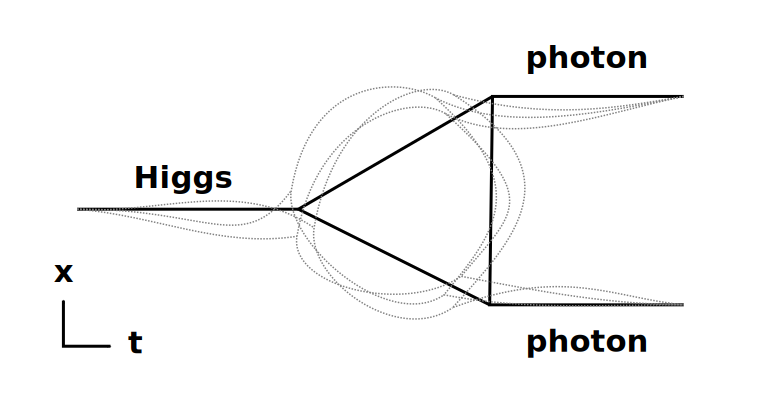
\includegraphics[width=\linewidth]{higgs-to-gamma-gamma_diagram.png}
\end{columns}

\vfill
\includegraphics[width=0.6\linewidth]{higgs-to-gamma-gamma_100fb-1.png}
\end{frame}

\begin{frame}
\frametitle{Why do we need such high-energy collisions?}

\begin{columns}
\column{0.5\linewidth}
\includegraphics[width=\linewidth]{cross-sections.jpg}

\column{0.5\linewidth}
\begin{itemize}\setlength{\itemsep}{0.2 cm}
\item Plot of rates of various types of processes versus proton collision energy

\item Note that the vertical axis is a log scale: every tick-mark is a
  factor of 10

\item Also notice that Higgs is on the bottom, but rises quickly with
  proton collision energy

\item High energy dramatically increases the signal-to- background ratio
\end{itemize}
\end{columns}
\end{frame}

\beamertemplateshadingbackground{lightyellow}{lightyellow}
\begin{frame}
\frametitle{The Higgs isn't the whole story}
\begin{itemize}\setlength{\itemsep}{0.5 cm}
\item Theorists have had 35 years to think about the Standard Model; \\
  it is incomplete

\item The Higgs boson's {\it own} mass needs to be explained

\item ``Physics as we know it breaks down at energy scales of several
  TeV.  At that point, something new takes the place of the Standard
  Model.''

\item We provide the 14~TeV collisions, nature will do what it will
  do, and we have general-purpose detectors to analyze whatever that
  turns out to be

\item For the first time in a generation of physicists, we are
  stepping into the unknown\ldots

\end{itemize}
\label{numpages}
\end{frame}

\beamertemplateshadingbackground{white}{white}

%% \begin{frame}
%% \frametitle{Outline}
%% \begin{itemize}\setlength{\itemsep}{0.75 cm}
%% \item 
%% \end{itemize}
%% %% \hspace{-0.83 cm} \textcolor{darkblue}{\Large Outline2}
%% \end{frame}

%% \section*{First section}
\begin{frame}
\begin{center}
\Huge \textcolor{blue}{Backup Slides}
\end{center}
\end{frame}

\begin{frame}
\frametitle{We're not doomed}

\begin{columns}
\column{0.6\linewidth}
\includegraphics[width=\linewidth]{cosmics_spectrum.png}

\column{0.4\linewidth}
\begin{itemize}
\item The universe is raining 16 LHC-like proton collisions
  down on the Earth every millisecond
\end{itemize}

\includegraphics[width=\linewidth]{cosmic_ray_showers.jpg}
\begin{itemize}
\item And it has been for 4 billion years

\item At full luminosity, the LHC would need to run for 65,000 years
  to contribute significantly
\end{itemize}
\end{columns}
\end{frame}

\begin{frame}
\frametitle{Extra dimensions}
\begin{columns}
\column{0.35\linewidth}
\includegraphics[width=\linewidth]{extra_dimensions2.png}
\column{0.6\linewidth}
\begin{center}
?
\end{center}
\end{columns}
\end{frame}

\begin{frame}
\frametitle{Supersymmetry}
\includegraphics[width=\linewidth]{supersymmetry_unification.png}
\end{frame}

\begin{frame}
\frametitle{Unification}
\includegraphics[width=\linewidth]{super_unification.jpg}
\end{frame}

\begin{frame}
\frametitle{LHC tides}
\includegraphics[width=\linewidth]{lhc_tides.png}

\begin{itemize}
\item The tides have an already-observable effect on the LHC
\item When the size of the ring stretches, the protons' orbit is perturbed
\item Corrections are necessary
\end{itemize}
\end{frame}

\begin{frame}
\frametitle{ATLAS}
\includegraphics[width=\linewidth]{atlas_diagram.png}
\end{frame}

\begin{frame}
\frametitle{CMS}
\includegraphics[width=\linewidth]{cms_schematic.png}
\end{frame}

\begin{frame}
\frametitle{CMS}
\includegraphics[width=\linewidth]{cms_particles.png}
\end{frame}

\begin{frame}
\frametitle{ATLAS two-muon event}
\includegraphics[width=\linewidth]{atlas_dimuon.png}
\end{frame}

\begin{frame}
\frametitle{CMS two-muon event}
\includegraphics[width=\linewidth]{cms_dimuon.png}
\end{frame}

\begin{frame}
\frametitle{ATLAS}
\includegraphics[width=0.5\linewidth]{atlas2.jpg}
\end{frame}

\begin{frame}
\frametitle{ATLAS}
\includegraphics[width=\linewidth]{atlas3.jpg}
\end{frame}

\end{document}
